\section{Диффракция на щели}
По формуле:
\begin{equation}
    \cfrac{\sin \inner{\cfrac{d\pi}{\lambda}\sin{x}}}{\cfrac{d\pi}{\lambda}\sin{x}}
\end{equation}

Максимумы будут в:
\begin{equation}
    d\sin{\theta} = k \lambda \implies \theta = \arcsin{\cfrac{k\lambda}{d}}
\end{equation}
\begin{equation}
    \cfrac{\sin{\theta}}{\sqrt{1 - \sin^2 \theta}} = \cfrac{x}{l}
\end{equation}
Поэтому зная расположение пиков на камере можем найти расстояние

\begin{figure}[h]
    \begin{subfigure}{.5\textwidth}
        \centering
        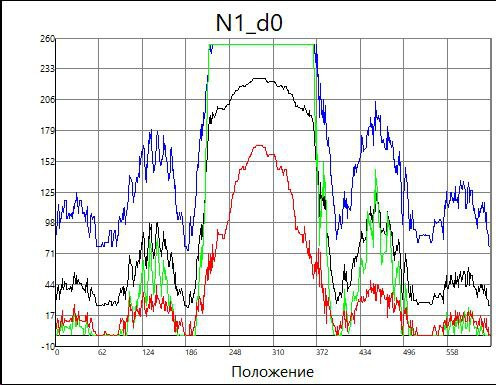
\includegraphics[trim={0 0 0 0},clip,width=\textwidth]{Ex_1/n1.jpg}
        \caption{}
        \label{n1}
    \end{subfigure}
    \begin{subfigure}{.5\textwidth}
        \centering
        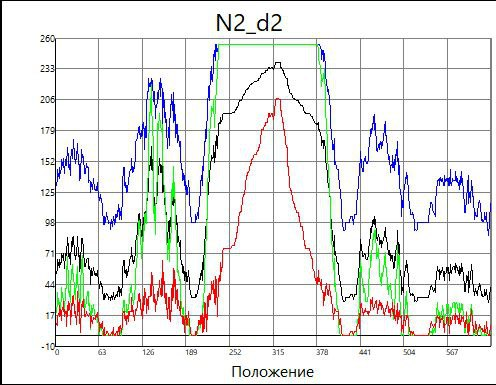
\includegraphics[trim={0 0 0 0},clip,width=\textwidth]{Ex_1/n2.jpg}
        \caption{}
        \label{n2}
    \end{subfigure}\\
    \begin{subfigure}{.5\textwidth}
        \centering
        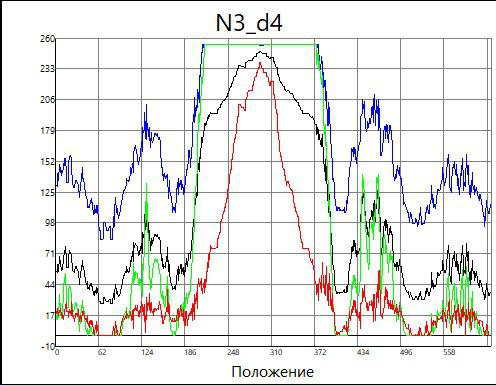
\includegraphics[trim={0 0 0 0},clip,width=\textwidth]{Ex_1/n3.jpg}
        \caption{}
        \label{n3}
    \end{subfigure}
    \begin{subfigure}{.5\textwidth}
        \centering
        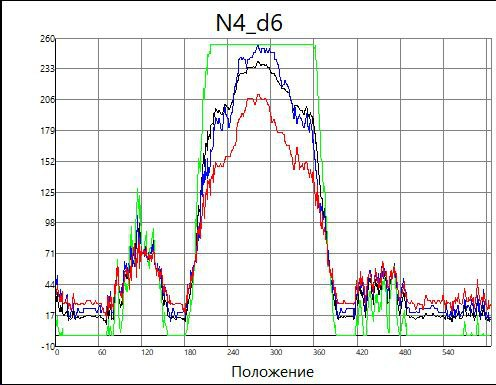
\includegraphics[trim={0 0 0 0},clip,width=\textwidth]{Ex_1/n4.jpg}
        \caption{}
        \label{n4}
    \end{subfigure}
\end{figure}







